% SOURCE: submissions/d2-neurocomputing/zenodo-deposit/results/merging/RG_gain_law_MERGED_REFIX20260730.json :: per-cell recomputed LOFO in-script (all-22 rho=-0.822, frozen <=-0.7; range [-0.85,-0.79] = most-negative to minimum-magnitude)
% !TEX encoding = UTF-8 Unicode
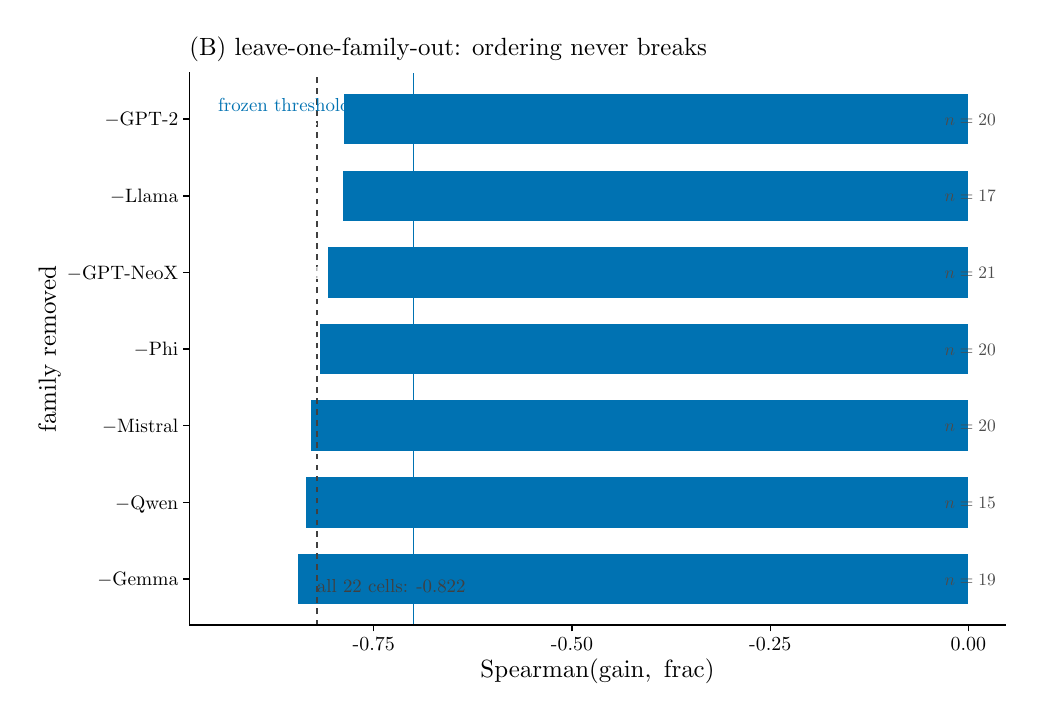
\begin{tikzpicture}[x=1pt,y=1pt]
\definecolor{fillColor}{RGB}{255,255,255}
\path[use as bounding box,fill=fillColor,fill opacity=0.00] (0,0) rectangle (361.35,238.49);
\begin{scope}
\path[clip] (  0.00,  0.00) rectangle (361.35,238.49);
\definecolor{drawColor}{RGB}{255,255,255}
\definecolor{fillColor}{RGB}{255,255,255}

\path[draw=drawColor,line width= 0.5pt,line join=round,line cap=round,fill=fillColor] (  0.00,  0.00) rectangle (361.35,238.49);
\end{scope}
\begin{scope}
\path[clip] ( 58.44, 22.61) rectangle (353.35,222.04);
\definecolor{fillColor}{RGB}{255,255,255}

\path[fill=fillColor] ( 58.44, 22.61) rectangle (353.35,222.04);
\definecolor{fillColor}{RGB}{0,114,178}

\path[fill=fillColor] ( 97.64, 30.09) rectangle (339.95, 48.37);

\path[fill=fillColor] (100.47, 57.78) rectangle (339.95, 76.07);

\path[fill=fillColor] (102.52, 85.48) rectangle (339.95,103.77);

\path[fill=fillColor] (105.53,113.18) rectangle (339.95,131.47);

\path[fill=fillColor] (108.47,140.88) rectangle (339.95,159.17);

\path[fill=fillColor] (113.80,168.58) rectangle (339.95,186.86);

\path[fill=fillColor] (114.15,196.28) rectangle (339.95,214.56);
\definecolor{drawColor}{gray}{0.25}

\path[draw=drawColor,line width= 0.5pt,dash pattern=on 2pt off 2pt ,line join=round] (104.52, 22.61) -- (104.52,222.04);
\definecolor{drawColor}{RGB}{0,114,178}

\path[draw=drawColor,line width= 0.5pt,line join=round] (139.36, 22.61) -- (139.36,222.04);
\definecolor{drawColor}{RGB}{255,255,255}

\node[text=drawColor,anchor=base east,inner sep=0pt, outer sep=0pt, scale=  0.68] at ( 95.47, 36.87) {-0.85};

\node[text=drawColor,anchor=base east,inner sep=0pt, outer sep=0pt, scale=  0.68] at ( 98.31, 64.57) {-0.84};

\node[text=drawColor,anchor=base east,inner sep=0pt, outer sep=0pt, scale=  0.68] at (100.36, 92.27) {-0.83};

\node[text=drawColor,anchor=base east,inner sep=0pt, outer sep=0pt, scale=  0.68] at (103.37,119.97) {-0.82};

\node[text=drawColor,anchor=base east,inner sep=0pt, outer sep=0pt, scale=  0.68] at (106.31,147.67) {-0.81};

\node[text=drawColor,anchor=base east,inner sep=0pt, outer sep=0pt, scale=  0.68] at (111.63,175.37) {-0.79};

\node[text=drawColor,anchor=base east,inner sep=0pt, outer sep=0pt, scale=  0.68] at (111.99,203.07) {-0.79};
\definecolor{drawColor}{gray}{0.30}

\node[text=drawColor,anchor=base west,inner sep=0pt, outer sep=0pt, scale=  0.63] at (331.35, 37.07) {$n=19$};

\node[text=drawColor,anchor=base west,inner sep=0pt, outer sep=0pt, scale=  0.63] at (331.35, 64.77) {$n=15$};

\node[text=drawColor,anchor=base west,inner sep=0pt, outer sep=0pt, scale=  0.63] at (331.35, 92.47) {$n=20$};

\node[text=drawColor,anchor=base west,inner sep=0pt, outer sep=0pt, scale=  0.63] at (331.35,120.17) {$n=20$};

\node[text=drawColor,anchor=base west,inner sep=0pt, outer sep=0pt, scale=  0.63] at (331.35,147.87) {$n=21$};

\node[text=drawColor,anchor=base west,inner sep=0pt, outer sep=0pt, scale=  0.63] at (331.35,175.57) {$n=17$};

\node[text=drawColor,anchor=base west,inner sep=0pt, outer sep=0pt, scale=  0.63] at (331.35,203.27) {$n=20$};
\definecolor{drawColor}{gray}{0.25}

\node[text=drawColor,anchor=base west,inner sep=0pt, outer sep=0pt, scale=  0.68] at (104.52, 34.21) {all 22 cells: -0.822};
\definecolor{drawColor}{RGB}{0,114,178}

\node[text=drawColor,anchor=base east,inner sep=0pt, outer sep=0pt, scale=  0.68] at (139.36,208.06) {frozen threshold <= -0.7};
\end{scope}
\begin{scope}
\path[clip] (  0.00,  0.00) rectangle (361.35,238.49);
\definecolor{drawColor}{RGB}{0,0,0}

\path[draw=drawColor,line width= 0.5pt,line join=round,line cap=rect] ( 58.44, 22.61) --
	( 58.44,222.04);
\end{scope}
\begin{scope}
\path[clip] (  0.00,  0.00) rectangle (361.35,238.49);
\definecolor{drawColor}{RGB}{0,0,0}

\node[text=drawColor,anchor=base east,inner sep=0pt, outer sep=0pt, scale=  0.70] at ( 54.39, 36.82) {$-$Gemma};

\node[text=drawColor,anchor=base east,inner sep=0pt, outer sep=0pt, scale=  0.70] at ( 54.39, 64.52) {$-$Qwen};

\node[text=drawColor,anchor=base east,inner sep=0pt, outer sep=0pt, scale=  0.70] at ( 54.39, 92.21) {$-$Mistral};

\node[text=drawColor,anchor=base east,inner sep=0pt, outer sep=0pt, scale=  0.70] at ( 54.39,119.91) {$-$Phi};

\node[text=drawColor,anchor=base east,inner sep=0pt, outer sep=0pt, scale=  0.70] at ( 54.39,147.61) {$-$GPT-NeoX};

\node[text=drawColor,anchor=base east,inner sep=0pt, outer sep=0pt, scale=  0.70] at ( 54.39,175.31) {$-$Llama};

\node[text=drawColor,anchor=base east,inner sep=0pt, outer sep=0pt, scale=  0.70] at ( 54.39,203.01) {$-$GPT-2};
\end{scope}
\begin{scope}
\path[clip] (  0.00,  0.00) rectangle (361.35,238.49);
\definecolor{drawColor}{RGB}{0,0,0}

\path[draw=drawColor,line width= 0.5pt,line join=round] ( 56.19, 39.23) --
	( 58.44, 39.23);

\path[draw=drawColor,line width= 0.5pt,line join=round] ( 56.19, 66.93) --
	( 58.44, 66.93);

\path[draw=drawColor,line width= 0.5pt,line join=round] ( 56.19, 94.63) --
	( 58.44, 94.63);

\path[draw=drawColor,line width= 0.5pt,line join=round] ( 56.19,122.32) --
	( 58.44,122.32);

\path[draw=drawColor,line width= 0.5pt,line join=round] ( 56.19,150.02) --
	( 58.44,150.02);

\path[draw=drawColor,line width= 0.5pt,line join=round] ( 56.19,177.72) --
	( 58.44,177.72);

\path[draw=drawColor,line width= 0.5pt,line join=round] ( 56.19,205.42) --
	( 58.44,205.42);
\end{scope}
\begin{scope}
\path[clip] (  0.00,  0.00) rectangle (361.35,238.49);
\definecolor{drawColor}{RGB}{0,0,0}

\path[draw=drawColor,line width= 0.5pt,line join=round,line cap=rect] ( 58.44, 22.61) --
	(353.35, 22.61);
\end{scope}
\begin{scope}
\path[clip] (  0.00,  0.00) rectangle (361.35,238.49);
\definecolor{drawColor}{RGB}{0,0,0}

\path[draw=drawColor,line width= 0.5pt,line join=round] (125.03, 20.36) --
	(125.03, 22.61);

\path[draw=drawColor,line width= 0.5pt,line join=round] (196.67, 20.36) --
	(196.67, 22.61);

\path[draw=drawColor,line width= 0.5pt,line join=round] (268.31, 20.36) --
	(268.31, 22.61);

\path[draw=drawColor,line width= 0.5pt,line join=round] (339.95, 20.36) --
	(339.95, 22.61);
\end{scope}
\begin{scope}
\path[clip] (  0.00,  0.00) rectangle (361.35,238.49);
\definecolor{drawColor}{RGB}{0,0,0}

\node[text=drawColor,anchor=base,inner sep=0pt, outer sep=0pt, scale=  0.72] at (125.03, 13.60) {-0.75};

\node[text=drawColor,anchor=base,inner sep=0pt, outer sep=0pt, scale=  0.72] at (196.67, 13.60) {-0.50};

\node[text=drawColor,anchor=base,inner sep=0pt, outer sep=0pt, scale=  0.72] at (268.31, 13.60) {-0.25};

\node[text=drawColor,anchor=base,inner sep=0pt, outer sep=0pt, scale=  0.72] at (339.95, 13.60) {0.00};
\end{scope}
\begin{scope}
\path[clip] (  0.00,  0.00) rectangle (361.35,238.49);
\definecolor{drawColor}{RGB}{0,0,0}

\node[text=drawColor,anchor=base,inner sep=0pt, outer sep=0pt, scale=  0.90] at (205.90,  3.75) {Spearman$(\mathrm{gain},\ \mathrm{frac})$};
\end{scope}
\begin{scope}
\path[clip] (  0.00,  0.00) rectangle (361.35,238.49);
\definecolor{drawColor}{RGB}{0,0,0}

\node[text=drawColor,rotate= 90.00,anchor=base,inner sep=0pt, outer sep=0pt, scale=  0.90] at ( 10.20,122.32) {family removed};
\end{scope}
\begin{scope}
\path[clip] (  0.00,  0.00) rectangle (361.35,238.49);
\definecolor{drawColor}{RGB}{0,0,0}

\node[text=drawColor,anchor=base west,inner sep=0pt, outer sep=0pt, scale=  0.90] at ( 58.44,228.29) {(B) leave-one-family-out: ordering never breaks};
\end{scope}
\end{tikzpicture}
